\newpage
\section{星系群与星系团}
\small
星系群/团是目前宇宙中常见的自引力束缚结构, 是星系、黑洞、气体、暗物质演化和极端天文现象的重要场所, 无论是对于星系形成, 还是宇宙学研究, 星系群/团都具有重要的地位, 一直是天文的重要研究对象. 
\normalsize
\subsection{星系群/团的基本观测性质}
\begin{itemize}\small
    \item 星系群(Galaxy group) 和星系团(Galaxy cluster)是星系密度较高的区域. 观测发现宇宙中有大约50\%的星系都处于星系群/团中, 其典型尺度$\sim$1 Mpc, 星系密度为宇宙星系平均密度的10$\sim$100倍
    \item  星系群/团是宇宙中的典型结构, 已经脱离了宇宙膨胀, 而处于自身引力势主导的演化阶段. 
    \item 星系团是宇宙中年轻的结构. 其成员星系的典型速度500km/s, 穿越整个星系团(直径3Mpc)的时间$\sim$8Gyrs. 因此大部分成员星系都还没有完成一个轨道周期, 无法与其他星系交换速度, 达到完全动力学平衡. 
    \item 并没有严格的区分星系群/星系团的定义. 一般来说
    \subitem 星系群的成员星系$<50$, 暗物质质量$[10^{12}, 10^{14}]M_{\odot}$
    \subitem 星系团质量$>10^{14} M_{\odot}$, 最大超过$10^{15} M_{\odot}$, 是目前宇宙中能形成的最大的引力束缚结构
\end{itemize}

\subsubsection{星系群---盘星系之家}
星系群中一般只有$\sim$10-30个星系, 一般包含几个与银河系或特征亮度($L^*$)接近的星系($\sim10^{10} L_{\odot}$). 其中成员星系以漩涡/盘星系居多成员星系平均速度弥散度$\sim$150-300km/s, 空间尺度从50$\sim$500 Kpc. 

星系群可以分为:
\begin{enumerate}\small
    \item Poor group (松散星系群): 含有少于5个$L^*$的成员星系, 分布在较大空间范围内 (银河系所在的近邻星系群就说Poor cluster)
    \item Compact group(紧密星系群): 成员星$\sim$几个, 分布紧密. Paul Hickson创建了一个Compact Group的星表, 简称Hickson Compact Groups. 一般认为Compact group处于动力学演化之中, 星系之间有很强的相互作用. 
    \item Fossil group(化石星系群): 典型特征
    \subitem 成员星只有几个, 中间为一个大质量椭圆星系. 中心椭圆星系与最亮的卫星星系之间的星等差$\Delta M > 2$ (质量差$\sim$10倍)
    \subitem 具有延展的高温气体, 温度$\sim$1000万度, 在X-ray波段可以看到热气体分布在椭圆星系周围
    \subitem 含有大量暗物质
    \subitem Fossil group是星系群演化到后阶段的结果, 大部分成员星系已经与中央星系并和, 形成了中心大质量椭圆星系. 因此是古老的星系群结构(Fossil group). 
\end{enumerate}
动力学摩擦效应: 质量越大的卫星星系, 其收到的动力学摩擦越强, 更快落入星系群中心, 与中央星系并和, 形成椭圆星系. 因此经过较长时间演化以后, 大质量卫星星系都已经消失, 形成大的星等差(Gap). 

\subsubsection{星系团---椭圆星系, 不规则星系之家}
星系团是宇宙中的``大个子''. 其中包含星系超过100个, 最多几千个. 典型半径$\sim$1-3 Mpc,星系的典型运动速度800-1200km/s. 近邻宇宙附近有名的星系团: VirgoCluster(室女星系团), Fornax Cluster(天炉座星系团), Coma(后发座星系团). 它们的成员星系都超过1000. 

星系团中心一般都有一个大质量椭圆星系. 如M87( Virgo cluster中心星系),其包含15000个球状星团(银河系$\sim$200个), 总恒星质量$\sim  10^{12} M_{\odot}$. 几乎所有的椭圆星系中心都有一个超大质量黑洞, 如M87的黑洞质量$\sim 6*10^9 M_{\odot}$, 同时在射电波段可以看到很强的物质喷流(外流速度$>$1000km/s, 空间尺度上百万光年).星系团中央星系非常延展, 其恒星分布接近50$\sim$100 Kpc, 恒星密度在外围较低, 接近星系间恒星(intra-cluster light, ICL)的背景密度, 因此中心星系的质量测量存在不确定性. 

\paragraph{星系团的X射线图像}
星系团中都含有大量的热气体, 在X射线波段发出辐射. 

\subsubsection{星系的演化}
星系团中星系密度高, 因此星系的演化明显与孤立星系不一样. 观测表明对于星系团, 存在一些明显的环境效应. 
\begin{enumerate}\small 
    \item 星系形态-密度关系(Morphology-density relation)
    \begin{itemize}
        \item 在星系团中心, 星系密度高, 椭圆星系比例高, 其比例随着半径增加而减小
        \item 在星系外围, 漩涡星系和不规则星系比例增加. 
    \end{itemize}
    \subitem 一般认为, 在星系团中心, 星系之间发生频繁的碰撞、并和, 形成了椭圆星系. 同时, 被瓦解星系的恒星分布在较大空间范围, 导致中央星系的恒星分布延展. 
    \subitem 后来的研究利用SDSS发现, 该morphology-density效应普遍存在于任何区域. 
    \item Butcher-Oemler effect: 在研究远距离(中等红移, z$\sim$0.3)的星系团时, Butcher \& Oemler(1978)发现星系团中蓝星系的比例比目前宇宙(z$\sim$0)中星系团的蓝星系比例高
    \subitem 目前观测发现, 这是一个普遍规律. 在早期宇宙, 几乎在所有环境中, 蓝星系的比例都高. 
    \item 光度函数-星系团质量关系: 通过测量不同质量星系团中, 不同类型星系的数目分布发现
    \begin{itemize}
        \item 高亮度处, 椭圆星系占大部分
        \item 低亮度处, 矮椭圆/不规则星系的数目占主导    
    \end{itemize}
    该效应随着星系团质量而变化, 对于星系群, 其亮星系主要是漩涡星系和S0 
\end{enumerate}

\subsubsection{位力定理估计质量}
一般来说, 星系群/团整体相对观测者有一定的运动速度, 同时, 成员星系还相对于星系群/团运动, 因此实际测量到的成员星速度是两者叠加. 
\begin{figure}[!htb]
    \centering
    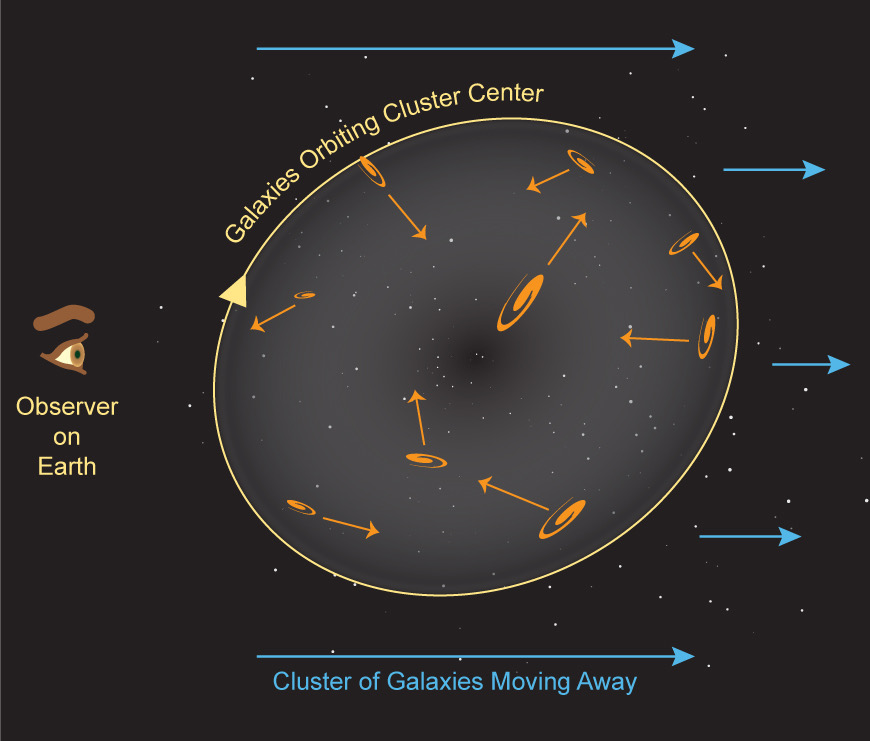
\includegraphics[width=0.309\textwidth]{GA6/成员星速度}
    \caption{成员星速度}
\end{figure}

通过测量单个成员星系的光谱, 可以得到其红移$z_i$, 对于$N$个成员星系, 可以得到星系群/团的平均红移
\begin{align*}
    \bar{z}=\frac{1}{N}\sum_{i=1}^N z_i
\end{align*}
进一步得到成员星系$i$相对系统整体运动速度(沿着视线方向)$V_i=c(z_i-\bar{z})$, $c$为光速. 

系统成员星系的平均速度(或速度弥散度)
\begin{align*}
    \sigma^2=\braket{V^2}=\frac{1}{N}\sum_{i=1}^N V_i^2
\end{align*}

\paragraph{位力定理}
成员星系的平均动能
\begin{align*}
    E=\frac{3}{2}\sigma^2 \cong \frac{GM}{R}
\end{align*}
$M$为星系群/团总质量, $R$为系统典型尺寸. 

\begin{figure}[!htb]
    \centering
    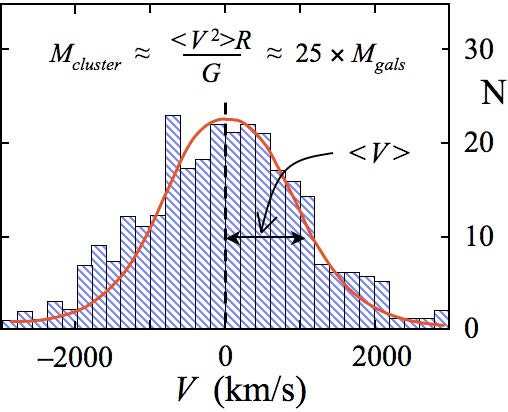
\includegraphics[width=0.309\textwidth]{GA6/成员星系的平均动能}
    \caption{成员星系的平均动能}
\end{figure}

\begin{itemize}\small
    \item 典型星系群, 速度弥散$\sigma \sim $300km/s, 半径300Kpc,则$M\sim 10^{13} M_{\odot}$
    \item 典型星系团, $\sigma \sim $1000km/s, 半径1000Kpc, 则$M\sim 4*10^{14} M_{\odot}$
\end{itemize}

\paragraph{温度-速度弥散关系}
对于处于维里化的星系团, 假设气体原子的平均速度与星系的速度弥散度相当. 对于气体粒子, 其能量
\begin{align*}
    \epsilon=\frac{3}{2}\kappa_B T
\end{align*}
$\kappa_B$为玻尔兹曼常数 = $1.38*10^{-23} $ J/K. 如果气体完全电离, 且主要成分为氢, 其动能
\begin{align*}
    K=\frac{3}{2}m_p\sigma^2
\end{align*}
这里为$\frac{3}{2}$,因为$\sigma$是沿着视线方向的速度, 为1维, 在均匀各向同性假设下, 3D速度 $v^2= 3\sigma^2$, $m_p$ 为质子质量 $= 1.67 * 10^{-27} $kg. 由$\epsilon=K$, 可得
\begin{align*}
    T=\frac{\frac{m_p}{2}\sigma^2}{\kappa_B}=5*10^6\left( \frac{\sigma}{300\text{km/s}} \right)^2
\end{align*}
\begin{itemize}\small
    \item $\sigma$=300km/s, $T$=500万度
    \item $\sigma$=1000km/s, $T$=4500万度. 
\end{itemize}
在这样的高温下, 气体完全电离, 主要辐射集中在x-ray波段($\sim$0.01-10 nm or 0.1keV $\sim$ 100 keV)

轫致辐射: 自由电子在库仑力作用下产生加速度, 辐射高能光子. 星系团的速度弥散与气体温度存在很好的相关关系. 基本符合维里定理. 


\subsubsection{冲压剥离 (ram-pressure stripping, RPS)}
当星系在星系团中运动时, 由于星系团内存在大量气体(星系际介质, Intracluster medium, ICM), 因此星系将感受到一个冲击压力(ram pressure), 就像骑车或者迎风打雨伞感受到阻力一样. 

\begin{figure}[!htb]
    \centering
    \begin{tikzpicture}
        \draw [fill=light_blue] (0,0) circle (2) node [white] {星系团};

        \coordinate (C) at (0.8, 1.2);
        \draw[light_red, ->, thick] (C)--(-0.4, 1) node [midway, above] {$V$};
        \draw [fill=light_red] (C) circle (0.32) node [white] {$R$};
    \end{tikzpicture}
\end{figure}

对于一个半径为$R$的星系, 以速度$V$在星系团中运动, 其单位时间内与该星系碰撞的气体质量为$\pi R^2 \rho_{ICM}V$, 由于星系对ICM的阻挡, 其感受的动量$\sim \pi R^2\rho_{ICM}V^2$ , 即单位面积受到的压强为$\rho_{ICM}V^2$. 

对一个无限薄盘, 如果其物质密度主要由恒星主导, 恒星面密度为$\Sigma^*$,  则其在距离盘面垂直距离$z$处的引力指向盘面, 为$2\pi G\Sigma^*$ . 则盘中气体单位面积的引力为$2\pi G \Sigma^* \Sigma_{ISM}$, 发生冲击压剥离的条件为$\rho_{ICM}V^2>2\pi G\Sigma^* \Sigma_{ISM}$, 即
\begin{align*}
    \rho_{ICM}>\frac{2\pi G \Sigma^* \Sigma_{ISM}}{V^2}
\end{align*}

对于一个类似银河系的星系, 其恒星质量$\sim 5*10^{10} M_{\odot}$ , 气体质量$5*10^9 M_{\odot}$ ,  分布在一个半径10kpc的盘面, 如果运动速度1000km/s, 则发生冲击压剥离的条件为$\rho_{ICM}>4*10^{-27}$g/cm${}^3$, 刚好接近星系团中ICM的平均密度. 

\begin{itemize}\small
    \item 在星系团中心, ICM的密度更高, 因此更容易发生RPS
    \item 星系外围, 气体和恒星密度低, 也容易发生RPS    
\end{itemize}

\subsection{引力透镜效应(Gravitational lensing)}
引力透镜是一种较常见的现象,它指光线穿过一个引力场附近时会发生弯曲的现象. 引力透镜已经成为测量天体物质分布, 宇宙学参数的标准手段(相比其他测量, 如位力定理, 需要假设其处于平衡态, 且需要光谱测量). 透镜现象只依赖于总物质分布, 是最``干净''的方法. 

按照透镜信号强弱, GL分为: 
\begin{itemize}
    \item 强引力透镜
    \item 弱引力透镜
\end{itemize}

\subsubsection{强引力透镜效应(Strong Gravitational lensing)}

\begin{figure}[!htb]
    \centering
    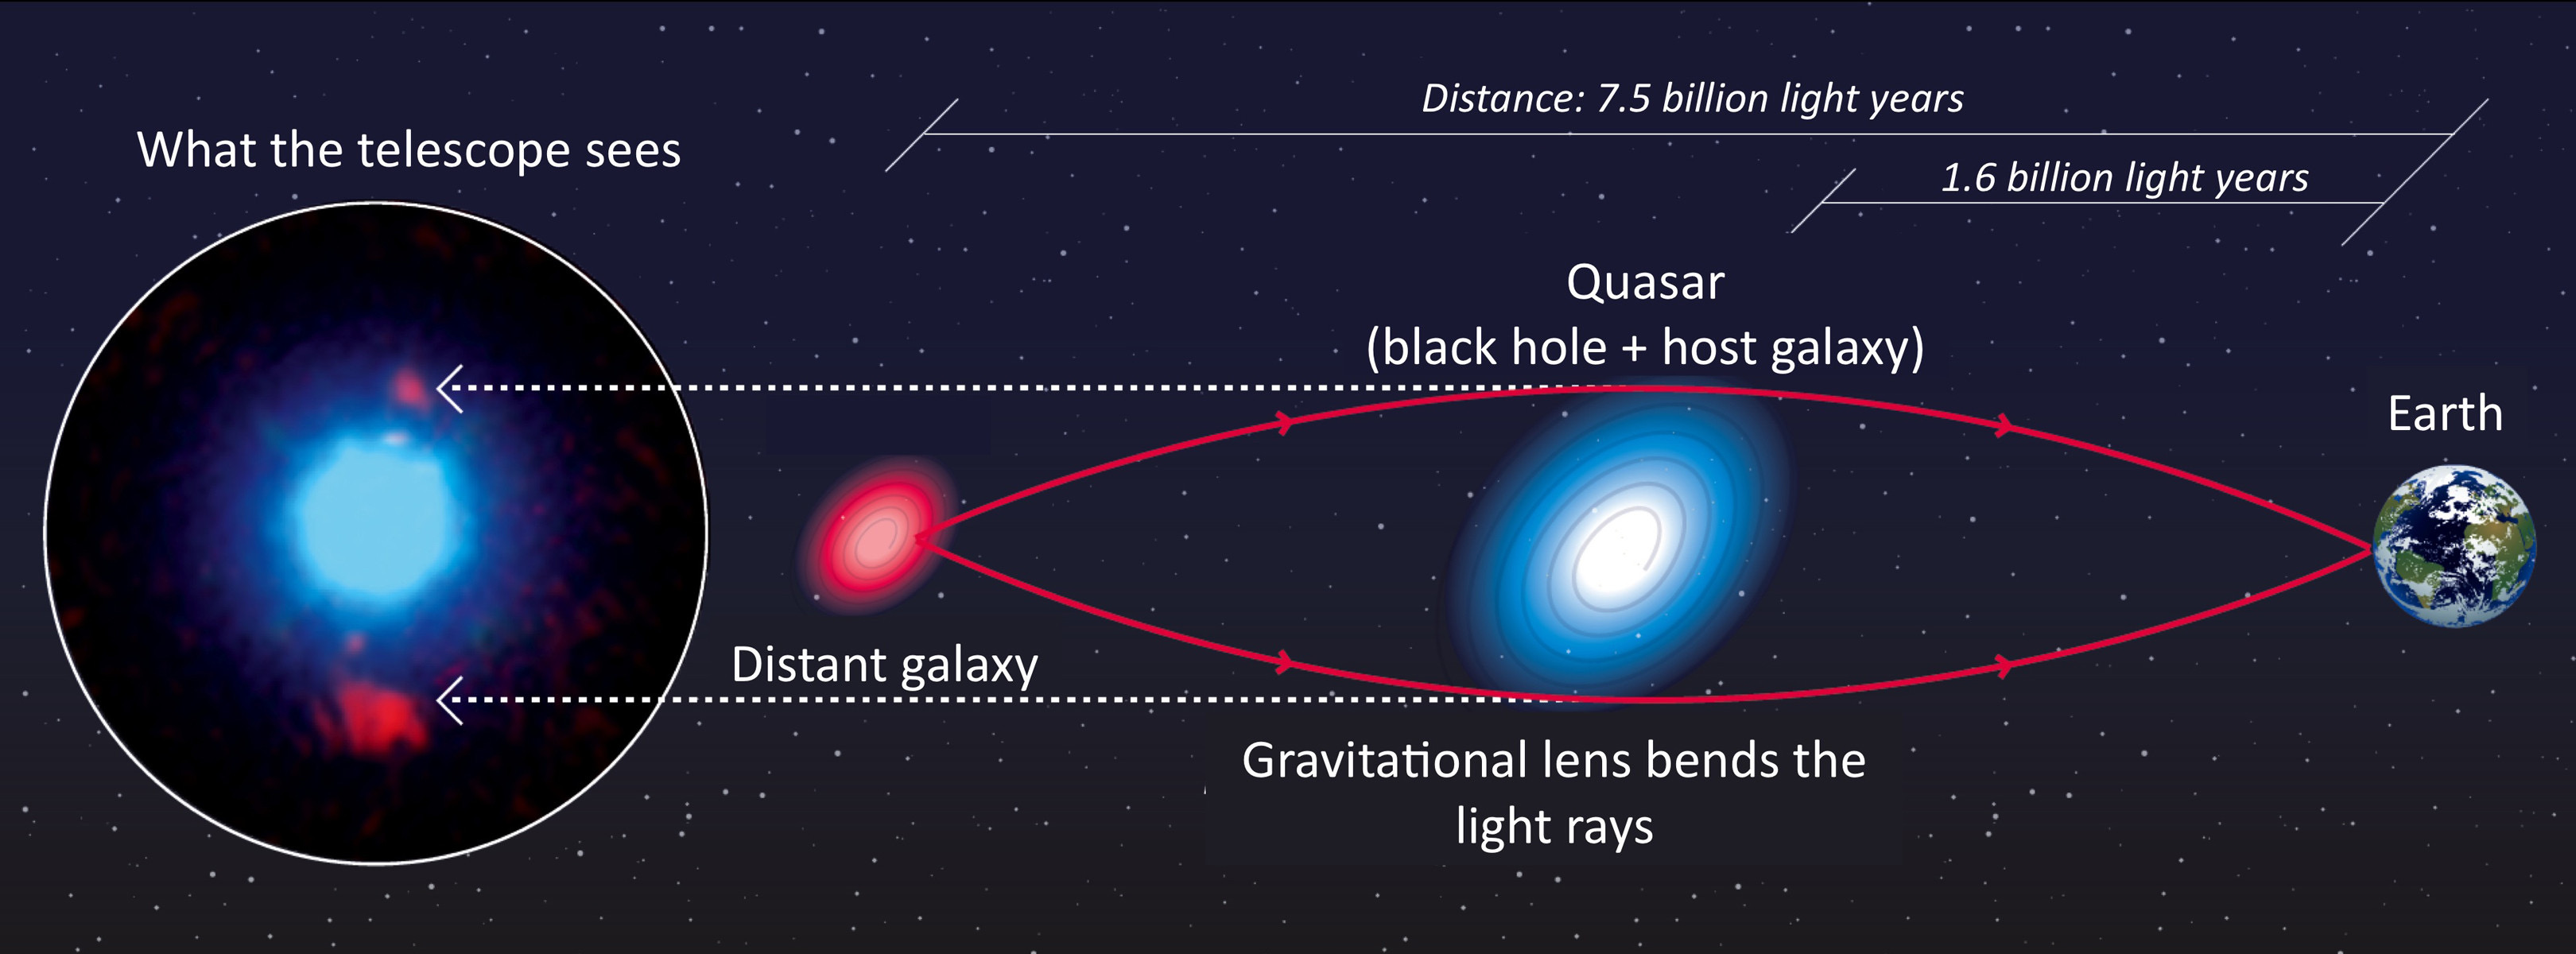
\includegraphics[width=0.47\textwidth]{GA6/强引力透镜效应}
    \caption{强引力透镜效应}
\end{figure}

基本原理: 背景星系(Source)的光被前景(Lens)弯曲,导致像的位置偏离真实位置, 并且可以成多个像. 

根据下图, 有如下等式
\begin{align*}
    d_s \theta =d_s \beta+d_{LS}\alpha
\end{align*}
\begin{figure}[!htb]
    \centering
    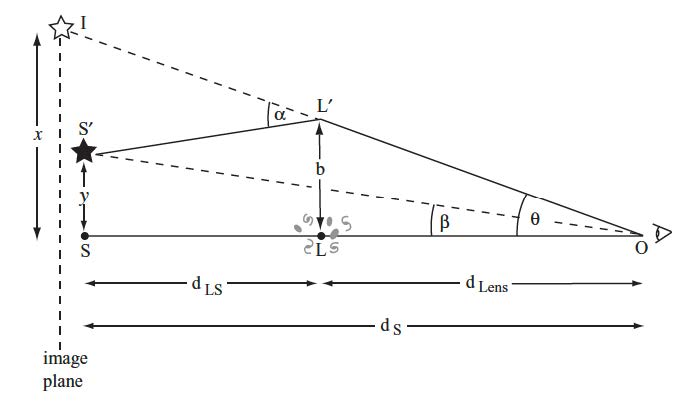
\includegraphics[width=0.36\textwidth]{GA6/强引力透镜}
    \caption{强引力透镜}
\end{figure}
在透镜$L$为点质量的情况下, 其偏折角$\alpha$可以从牛顿力学得到: 
\begin{align*}
    \alpha=\frac{2GM}{bc^2}
\end{align*}
实际上, 广义相对论给出
\begin{align*}
    \alpha=\frac{4GM}{bc^2}
\end{align*}

由上式可得 ($b=d_{lens}\theta$)
\begin{align*}
    \theta-\beta=\frac{1}{\theta}\frac{4GM}{c^2}\frac{d_{LS}}{d_s d_{lens}}=\frac{1}{\theta}\theta_E^2
\end{align*}
可求解得到
\begin{align*}
    \theta_{\pm}=\frac{\beta \pm \sqrt{\beta^2+4\theta_E^2}}{2}
\end{align*}
$\displaystyle\theta=\sqrt{\frac{4GM}{c^2}\frac{d_{LS}}{d_s d_{lens}}}$ 为爱因斯坦半径, 其大小与源, 透镜和观测者之间的距离和源的质量决定. 

\begin{itemize}\small
    \item 当$\beta=0$时, 即当源, 透镜和观测值成一条直线时,  $\theta=\theta_E$, 此时, 像为一个圆环, 其半径为爱因斯坦半径. 
    \item 当$\beta>0$, 有两个解, 分别在透镜的两侧, 位于爱因斯坦半径内外. 
\end{itemize}

\paragraph{放大效应}
对于上述点质量透镜情况, 它不但引起2个像, 同时还放大/减小源的表面积. 透镜引起源中心从$y(\beta)\rightarrow x(\theta)$, 同时径向尺度也发生变化. 由于源的表明亮度与距离无关, 因此像的面积相对于源的面积变化引起总亮度变化. 

\begin{figure}[!htb]
    \centering
    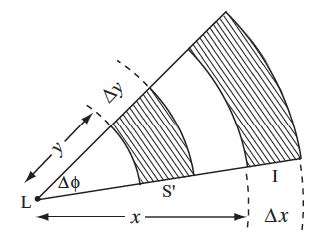
\includegraphics[width=0.24\textwidth]{GA6/放大效应}
    \caption{放大效应}
\end{figure}

\begin{align*}
    \frac{\mathcal{A}_\pm (image)}{\mathcal{A}(source)}&=\left| \frac{\theta}{\beta}\frac{d\theta}{d\beta} \right|\\
    &=\frac{1}{4}\left( \frac{\beta}{\sqrt{\beta^2+4\theta_E^2}}+\frac{\sqrt{\beta^2+4\theta_E^2}}{\beta}\pm 2 \right)
\end{align*}
可以看出, 
\begin{itemize}\small
    \item 对于远离透镜的像$\theta_+$, 其放大率始终$>1$, 即该像始终变亮. 
    \item 对于靠近透镜的像$\theta_{-}$, 当$\beta\le 0.35\theta_E$时, 放大率$>1$, $\beta$偏大时放大率$<1$, 像变弱. 
\end{itemize}
两个像的总亮度为 $\mathcal{A}_++\mathcal{A}_->1$, 因此总亮度始终放大. 

当$\beta=\theta_E$ 时, 放大$\sim 40\%$, $\beta=0.7\theta_E$ , 放大1倍. 

\subsubsection{弱引力透镜效应( Weak Gravitational lensing)}
对于绝大多数情况, 透镜体不是点质量, 同时源处于距离透镜中心较远的位置时, 并不产生多个像, 源的位置基本不变化, 但是源的形状有轻微改变. 此为弱引力透镜效应. 

假如源为一个圆形, 则像的形状不但变大, 同时具有一定的椭率如下图所示. 
\begin{figure}[!htb]
    \centering
    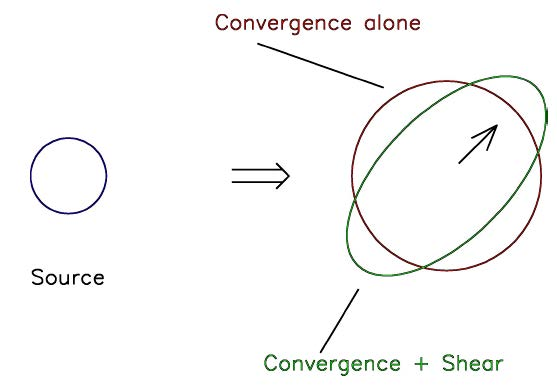
\includegraphics[width=0.309\textwidth]{GA6/弱引力透镜效应}
    \caption{弱引力透镜效应}
\end{figure}

弱引力透镜的比强引力透镜更加普遍, 且能测量到星系团外围的物质分布(强透镜只能测量中心到像之间的物质分布), 因此弱引力透镜在宇宙学中有非常重要的应用. 

\subsubsection{引力透镜效应总结}
\begin{itemize}\small
    \item 强引力透镜
    \subitem 源靠近透镜中心时产生
    \subitem 产生多个像
    \subitem 不同的像亮度不一样, 总体变亮
    \item 弱引力透镜
    \subitem 源偏离透镜中心
    \subitem 像的形状发生改变, 变得更加椭圆
\end{itemize}
两者都可以用来测量透镜体的物质分布同时, 由于放大效应, 可以较容易观测到很远的源. 

\subsection{星系团SZ现象}
SZ效应指宇宙微波背景辐射的光子在穿过星系团时, 由于星系团内的高能电子与光子发生逆康普顿散射, 由于电子具有较高能量, 散射后光子获得能量. 

首先考虑康普顿散射, 即光子与静止电子发生散射
\begin{figure}[!htb]
    \centering
    \begin{tikzpicture}
        \draw[fill=light_blue] (0, 0) circle (0.2);


        \draw[draw=light_blue, ->] (-2, 0) node [below] {$\nu_i$}--(-0.2, 0);
        \draw[draw=light_blue, ->] (30:0.2)--(30:1.2) node [above] {$v$};
        \draw[draw=light_red, ->] (-30:0.2)--(-30:1.8) node [below] {$\nu$};
        \draw[draw=light_blue, dashed] (0.2, 0)--(1.8, 0) node [midway, above] {$\varphi$} node [midway, below] {$\theta$};
    \end{tikzpicture}
\end{figure}
入射光子频率$\nu_i$, 散射光子频率$\nu$, 散射后电子速度$v$. 

散射过程满足以下方程:
\begin{enumerate}
    \item 能量守恒
    \begin{align*}
        h\nu_i +m_e c^2=h\nu + m_e c^2 \gamma
    \end{align*}
    洛伦兹因子$\displaystyle\gamma=\frac{1}{\sqrt{1-\left( \frac{v}{c} \right)^2}}$ 
    \item 动量守恒
    \begin{align*}
        \frac{h\nu_i}{c}=\frac{h\nu}{c}\cos\theta +m_e v\gamma \cos\varphi &\text{ (水平方向)} \\
        \frac{h\nu}{c}\sin\theta=m_e v\gamma \sin\varphi &\text{ (垂直方向)}
    \end{align*}
\end{enumerate}

求解上述方程, 可以得到散射前后光子的频率为
\begin{align*}
    \nu=\frac{\nu_i}{1+\frac{h\nu_i}{m_e c^2}(1-\cos\theta)}
\end{align*}
可以看到, 光子与静止电子碰撞后, 光子能量变小, 电子获得能量. 

\begin{figure}[!htb]
    \centering
    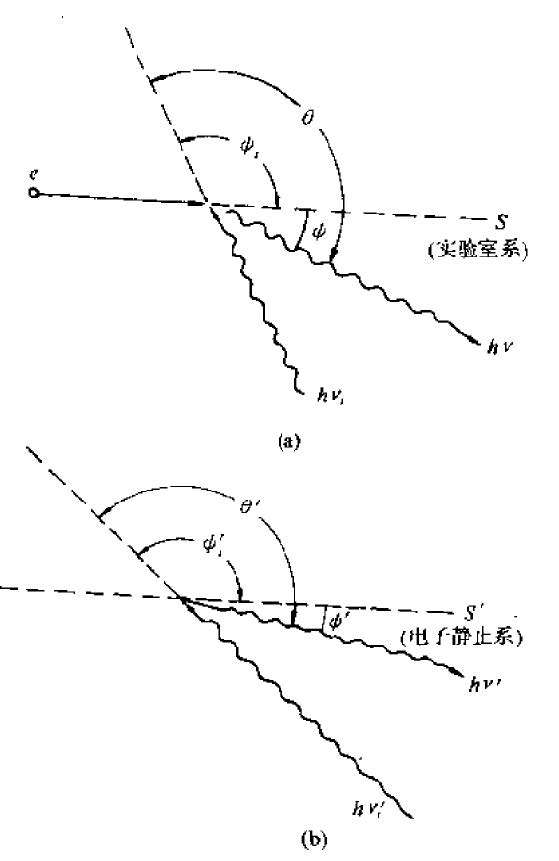
\includegraphics[width=0.24\textwidth]{GA6/逆康普顿散射}
    \caption{逆康普顿散射}
\end{figure}

当电子能量相比入射光子能量较高时, 散射后光子获得能量, 称为逆康普顿散射. 有如下推导: 

在电子的静止坐标系内$S'$, 入射光子和散射光子频率满足上式, 此时用电子静止坐标系中的频率代替
\begin{align*}
    \nu'=\frac{\nu'_i}{1+\frac{h\nu'_i}{m_e c^2}(1-\cos\theta')}
\end{align*}
要从电子静止坐标系$S'$变换到实验室坐标系$S$中, 需要利用相对论变化关系
\begin{itemize}\small
    \item $S\rightarrow S'$ 时, 入射光频率变换: $h\nu'_i=\gamma h\nu_i(1-\beta\cos\psi_i)$
    \item $S'\rightarrow S$ 时, 散射光频率变换: $h\nu=\gamma h\nu'(1+\beta \cos\psi')$
\end{itemize}
同时从$S\rightarrow S'$, 入射光和散射光角度的变化:
\begin{align*}
    \tan \psi'_i&=\frac{\sin\psi_i}{\gamma(\cos\psi_i-\beta)}\\
    \tan \psi'&=\frac{\sin\psi}{\gamma(\cos\psi-\beta)}
\end{align*}
代入上式可得
\begin{align*}
    h\nu=\frac{\gamma^2h\nu_i(1-\beta\cos\psi_i)(1+\beta \cos\psi')}{1+\frac{\gamma h\nu_i}{m_e c^2}(1-\beta\cos\psi_i)(1-\cos\theta')}
\end{align*}

考虑电子以相对论性速度运动(星系团中的电子), $\beta=\frac{v}{c}\simeq  1,\ \gamma\gg 1$. 即使如此, 对于X射线电子, 仍然有 $\gamma h \nu_i \ll m_e c^2$, 因此有
\begin{align*}
    h\nu \simeq \gamma^2 h\nu_i (1-\cos\psi_i)(1+\cos\psi')
\end{align*}
同时, $\psi\simeq 0$. 

平均来说, 在与相对论电子碰撞后, 散射光子基本沿着电子运动方向, 且能量增加了$\gamma^2$倍. 

\begin{figure}[!htb]
    \centering
    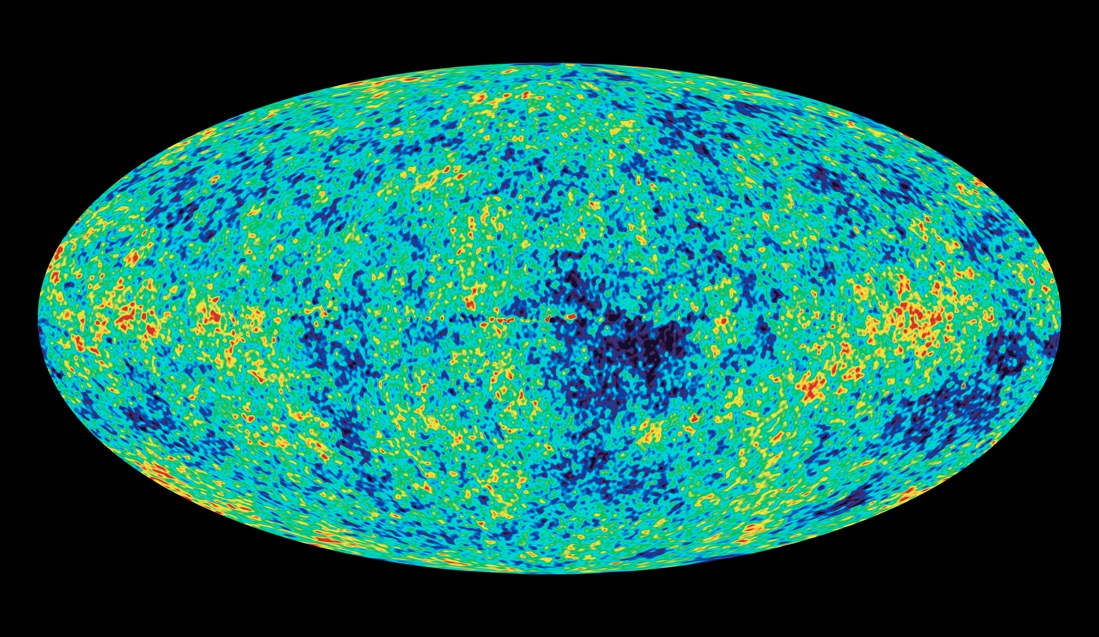
\includegraphics[width=0.309\textwidth]{GA6/宇宙背景辐射}
    \caption{宇宙微波背景辐射}
\end{figure}

对于宇宙背景辐射(CMB), 其为黑体谱, 其为
\begin{align*}
    I_{\nu}(\nu, T_{CMB})=\frac{2h\nu^3}{c^2}\frac{1}{e^{\frac{h\nu}{kT_{CMB}}}-1}
\end{align*}
Sunyaev-Zeldovich通过更加严格的推导得到电子对cmb能谱的改变为
\begin{align*}
    \frac{\Delta I_\nu}{I_\nu}=y\frac{xe^x}{(e^x-1)}\left[ x\left( \frac{e^x+1}{e^x-1} \right)-4 \right]
\end{align*}
康普顿散射光深 $y=\int \frac{K T_e}{m_e c^2}\sigma_T N_e dl$, $x=\frac{h\nu}{kT_r}$. 

可以看到, 光深正比于电子的动能$kT_e$ , 以及电子沿着视线方向的一维密度. 即星系团质量越大, 温度越高, SZ效应越强. 目前的观测表明光深$y$很小, $y\sim 10^{-5}$(尽管相对改变很小, 目前的天文观测精度足以测量出该效应). 

此外, 从上式对$x=\frac{h\nu}{kT_r}$的依赖关系可以看出, 能谱的改变依赖于光子的能量. 

下图显示CMB光子被热电子散射后能谱的改变
\begin{itemize}\small
    \item 在低能段($v<218$ GHz), 光子的总能量减小
    \item 在高能段($v>218$ GHz), 光子的总能量增加
\end{itemize}

\begin{figure}[!htb]
    \centering
    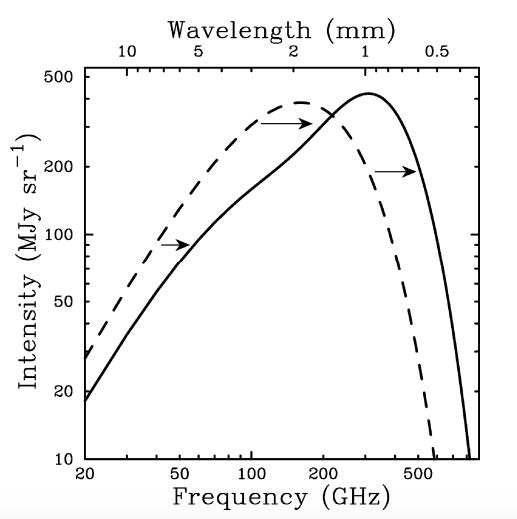
\includegraphics[width=0.309\textwidth]{GA6/CMB光子被热电子散射后能谱的改变}
    \caption{CMB光子被热电子散射后能谱的改变}
\end{figure}

SZ效应的最大优点是其对CMB光子能量的改变不依赖于星系团到我们的距离(星系团的光学或者X-ray辐射随着距离平方下降, 因此很难探测到较远距离), 因此广泛利用SZ效应寻找星系团. 

\small
提醒: 由于CMB本身在天空分布的不均匀性, 即使在某一区域探测到某个频率内CMB信号相对平均温度升高, 也不能说明该处存在星系团需要在几个不同的频率附近测量CMB的温度, 最好在218GHz左右分别测量几个频率. 
\normalsize